\chapter{Network Properties and Centrality Measures}

To fully characterize network properties, we evaluate measures that can be broadly divided into global and local categories.

\textbf{Global measures} evaluate the network as a whole entity, providing insights into its overall structure and behavior. These measures are crucial for understanding the macroscopic properties of the network and how it functions as a complete system. Examples of global features include:
\begin{itemize}
    \item The total number of nodes and edges, as well as the overall link density, which indicates how interconnected the network is.
    \item Structural metrics such as the diameter, girth, genus, and the total clustering coefficient, which provide insights into the network's topology and the presence of cycles and clusters.
    \item Spectral properties, which involve the analysis of the network's eigenvalues and eigenvectors, offering insights into its stability, robustness, and dynamic behavior.
    \item Assortativity and mixing patterns, which describe the tendency of nodes to connect with similar or dissimilar nodes based on certain attributes (e.g., degree, type).
    \item The presence and structure of network communities and motifs, which reveal the modular organization and recurring patterns within the network.
\end{itemize}

\textbf{Local measures}, conversely, focus on characteristics at the single node or edge level, or on the relationships between pairs of nodes or edges. These include:
\begin{itemize}
    \item Node and edge centrality measures, which assess the importance or influence of individual nodes or edges within the network.
    \item One-dimensional node or link feature distributions, such as degree distributions, which provide insights into the heterogeneity of connectivity.
    \item The relation between parameter distributions, often modeled as N-dimensional probability density functions (e.g., the joint distribution of degree and clustering coefficient), which can reveal correlations and dependencies between different local properties.
\end{itemize}

\subsubsection{Node and Link Centrality Measures}
Centrality measures are parameters that can be associated with every single node or link, or specific groups of them. They provide vital information regarding the relevance and importance of specific network elements and are typically characteristic of the type of network being considered.

These measures are particularly useful for:
\begin{itemize}
    \item Ranking and stratifying nodes and links based on their structural importance.
    \item Identifying peculiar elements, acting as outliers within the related statistical distributions of the network.
\end{itemize}

% ==========================================
\section{Degree Centrality}
% ==========================================

\textbf{Degree}, or connectivity, is a fundamental \textbf{local parameter}. It represents the total number of incoming or outgoing links connected to a specific node. In terms of linear algebra, for a directed network, this corresponds to the row or column sum of the adjacency matrix.

\begin{definition}[Degree]
    Let $K_{IN}(i)$ represent all the links entering the $i$-th node, and $K_{OUT}(i)$ represent all the links exiting the $i$-th node. They are defined as:
    \[ K_{IN} = \sum_{j} a_{ij}, \quad K_{OUT} = \sum_{i} a_{ij} \]
\end{definition}

For symmetric (undirected) networks, the adjacency matrix is equal to its transpose ($A = A^T$), meaning that $K_{IN} = K_{OUT}$. The underlying premise of degree centrality is straightforward: a node that is very connected is considered very important. Typical examples of this dynamic include website hyperlinks, academic citations, and friendship connections.

\subsection{Degree Distribution}
The \textbf{distribution of connectivity} across all nodes provides important information regarding the broader properties of the network. In particular, examining the heterogeneity of $K$ values, represented by the probability density function $p(k)$, helps characterize specific types of networks. Common types of degree distributions include:
\begin{itemize}
    \item \textbf{Poisson pdf:} Characteristic of the Erdős-Rényi (E-R) ensemble, often used as a baseline null model for random networks.
    \item \textbf{Scale-free pdf:} Characteristic of networks grown via preferential attachment, such as the Barabási-Albert (B-A) model, which leads to a power-law distribution of degrees.
    \item \textbf{Fat-tailed pdf:} Arises from several other complex stochastic processes.
\end{itemize}

\begin{example}[Human Protein Interaction Network]
    An excellent biological example of a non-trivial structure is the human Protein-Protein Interaction (PPI) network (e.g., PathwayCommons). This is a hierarchical network demonstrating a highly heterogeneous degree distribution that behaves very differently from a random E-R graph. The network is massive, consisting of more than 11,000 nodes and over 420,000 links , and is heavily characterized by a fat-tailed $p(k)$ distribution.
\end{example}
\begin{figure}[H]
    \begin{minipage}{0.4\textwidth}
        \caption{The human PPI network is a hierarchical network with a highly heterogeneous degree distribution, characterized by a fat-tailed $p(k)$ distribution. It consists of over 11,000 nodes and more than 420,000 links, demonstrating a structure that is very different from a random E-R graph.}
    \end{minipage}
    \hfill
    \begin{minipage}{0.55\textwidth}
        \centering
        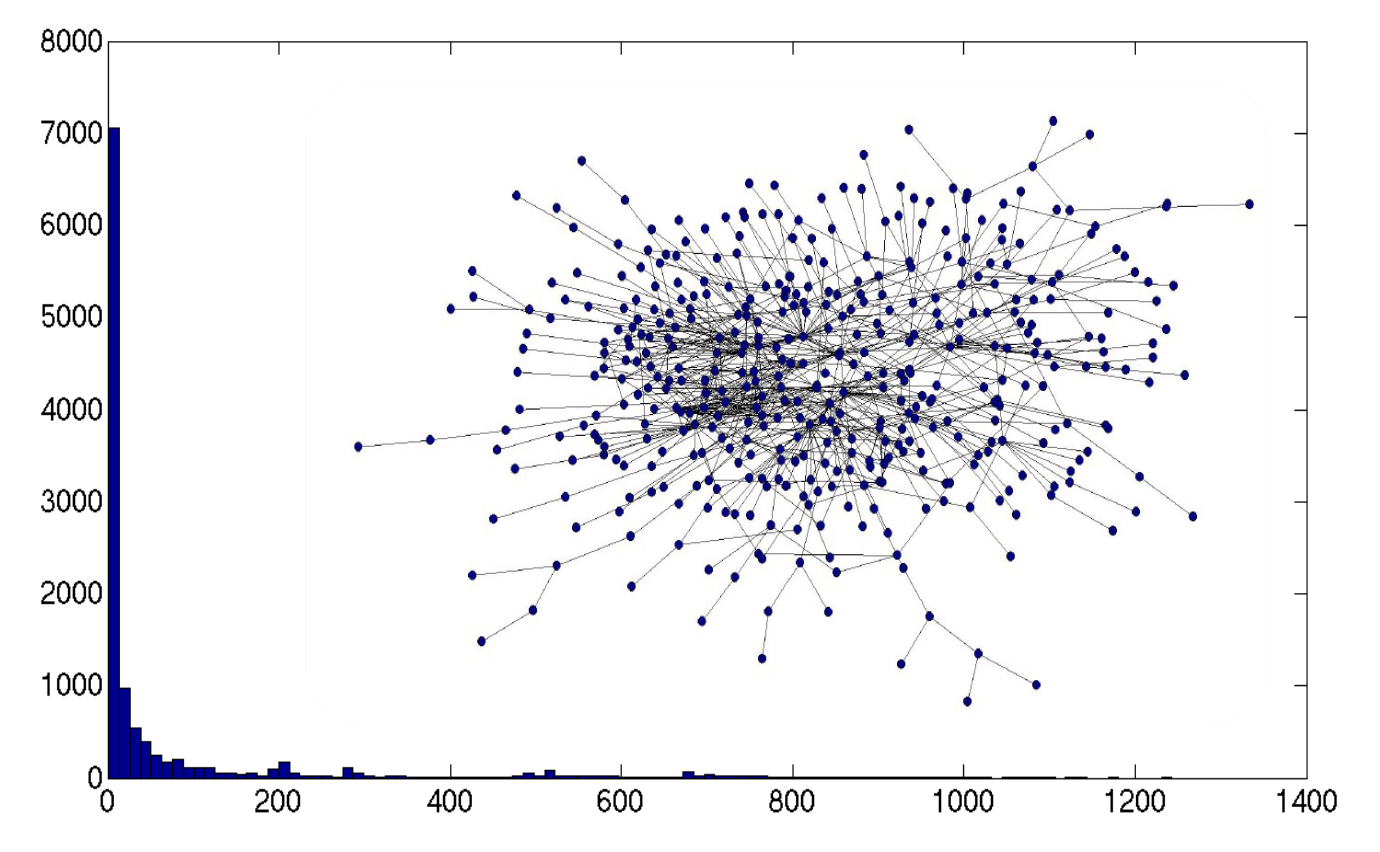
\includegraphics[width=\textwidth]{img/human_ppi_network.png}
    \end{minipage}
\end{figure}

\subsection{Multivariate Analysis of Degree}

In general, it is highly informative to consider the \textbf{joint distribution of couples of centrality measures}, often visualized using 2D histograms, density plots, or XY scatterplots. While some parameter pairs (e.g., \textit{betweenness centrality} vs. \textit{degree}) follow expected patterns defined by standard null models, non-trivial patterns frequently emerge in real networks, allowing us to identify interesting elements such as specialized nodes or links.

Erdős-Rényi (E-R) ensembles serve as the simplest null models to establish a baseline for these comparisons, as they are defined by a single parameter (the link density $\lambda$) and do not exhibit any correlations between node degrees.

Two standard 2D joint distributions analyzed are:
\begin{itemize}
    \item $K_{IN}$ vs $K_{OUT}$ (in a directed graph): in real networks (non E-R), we often observe non-trivial patterns that can indicate specific functional roles of nodes (e.g., "hubs" with high outdegree but low indegree).
    \item $K$ vs $K_{NN}$ (the average degree of a node's first neighbors): real networks often show significant correlations in this relationship, which can help identify specialized nodes (e.g., "effector" nodes with low degree but high-degree neighbors, or "master" nodes with high degree but low-degree neighbors).
\end{itemize}

\begin{definition}[Degree of Nearest Neighbors]
    The sum of the degrees of all first neighbors of node $i$ (i.e., nodes directly connected to the considered node) is:
    \[
        K_{NN}(i) = \sum_{i \sim j} K_j.
    \]
    The average degree of the nearest neighbors can be expressed as:
    \[
        \langle K_{NN}(i) \rangle = \frac{1}{N_{NN(i)}} \sum_{i \sim j} K_j,
    \]
    while, if we define the vector of degrees as $\vec{K} = (K_1, K_2, \ldots, K_N)$, we can express its nearest neighbor degree as a matrix operation:
    \[
        \vec{K}_{NN} = \sum_{j} A_{ij} \cdot K_j = A \cdot \vec{K} \oslash \vec{N},
    \]
    where $\oslash$ denotes the Hadamard (element-wise) division.
\end{definition}

\begin{example}[Joint Distributions in Null Models vs Real Networks]
    In an E-R directed random graph (our null model), there is no statistical relationship between indegree ($K_{IN}$) and outdegree ($K_{OUT}$), nor is there a relationship between a node's degree ($K$) and the degree of its neighbors ($K_{NN}$). The scatterplots appear uniform and uncorrelated.

    \begin{figure}[H]
        \begin{minipage}{0.6\textwidth}
            \centering
            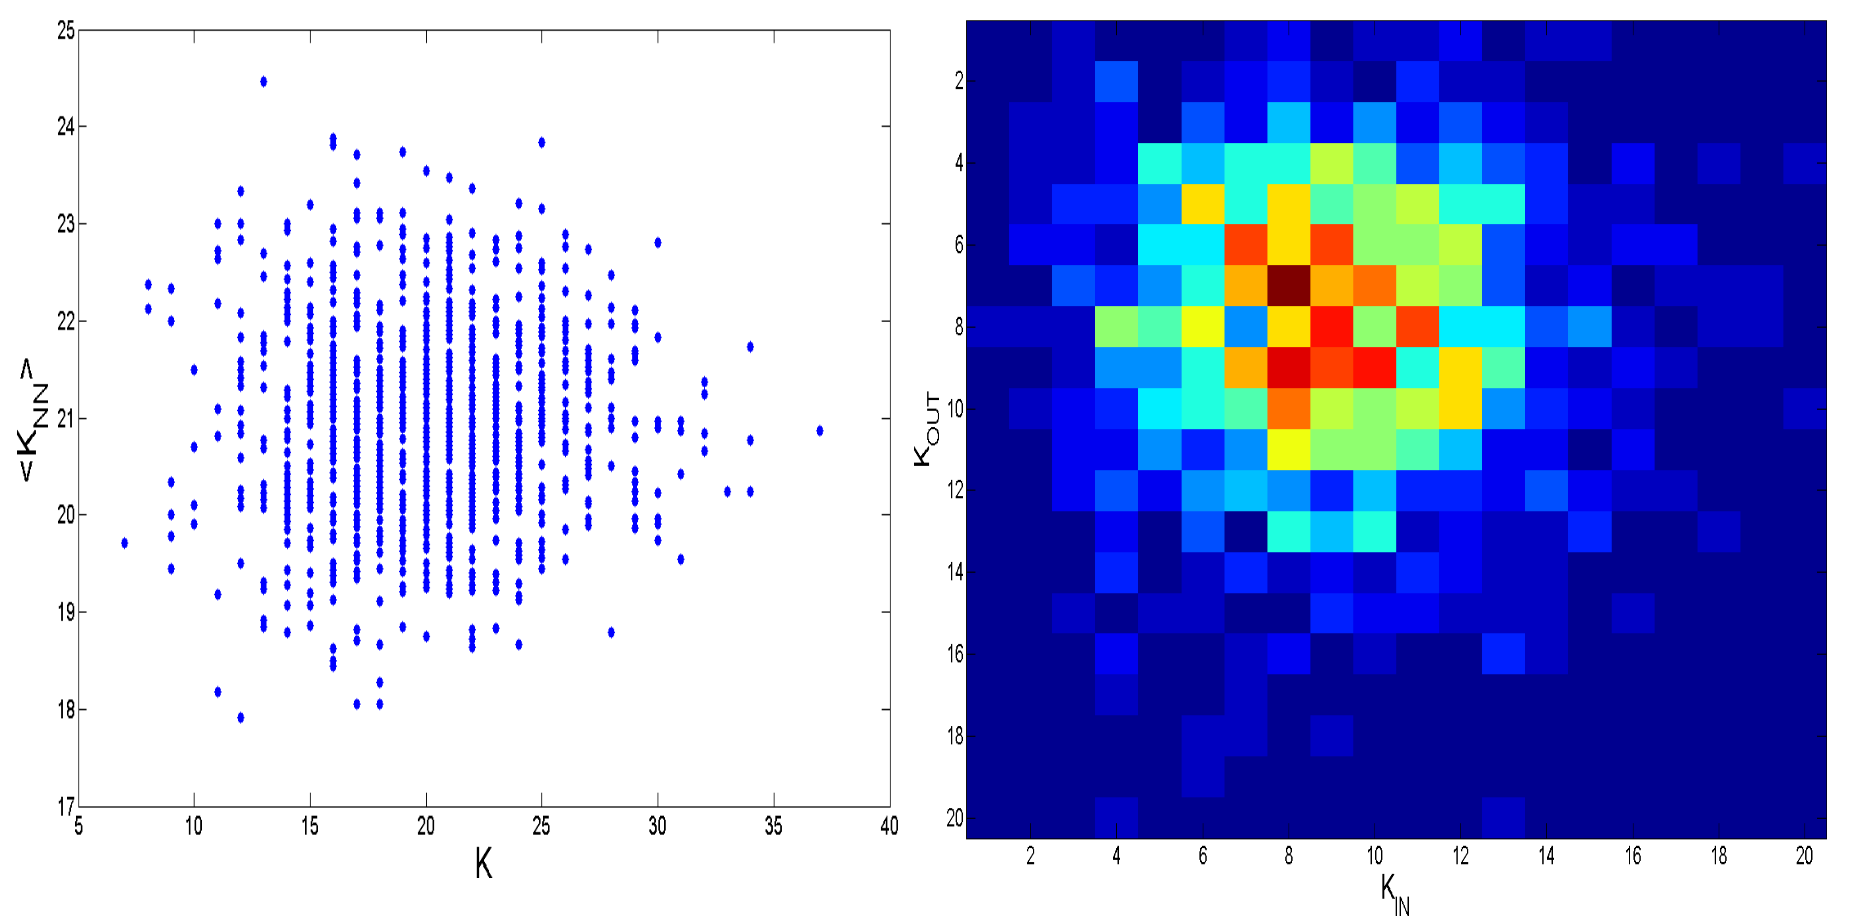
\includegraphics[width=\textwidth]{img/scatterplot-densityplot-ER.png}
        \end{minipage}
        \hfill
        \begin{minipage}{0.35\textwidth}
            \caption{In the left scatterplot of an E-R directed random graph, there is no statistical relationship between the NN degree ($K_{NN}$) and the node's degree ($K$), resulting in a uniform distribution. In the right one, the same happens with $K_{IN}$ and $K_{OUT}$.}
        \end{minipage}
    \end{figure}

    Conversely, biological networks like the Yeast PPI (Protein-Protein Interaction) network exhibit a non-trivial $K$ vs $K_{NN}$ correlation. This specific pattern helps identify specialized biological roles, such as "effector" and "master" nodes. If we perform a link reshuffling on this network (randomizing connections while preserving degrees), this observed pattern is completely destroyed, proving it is a product of evolutionary design rather than random chance.

    \begin{figure}[H]
        \centering
        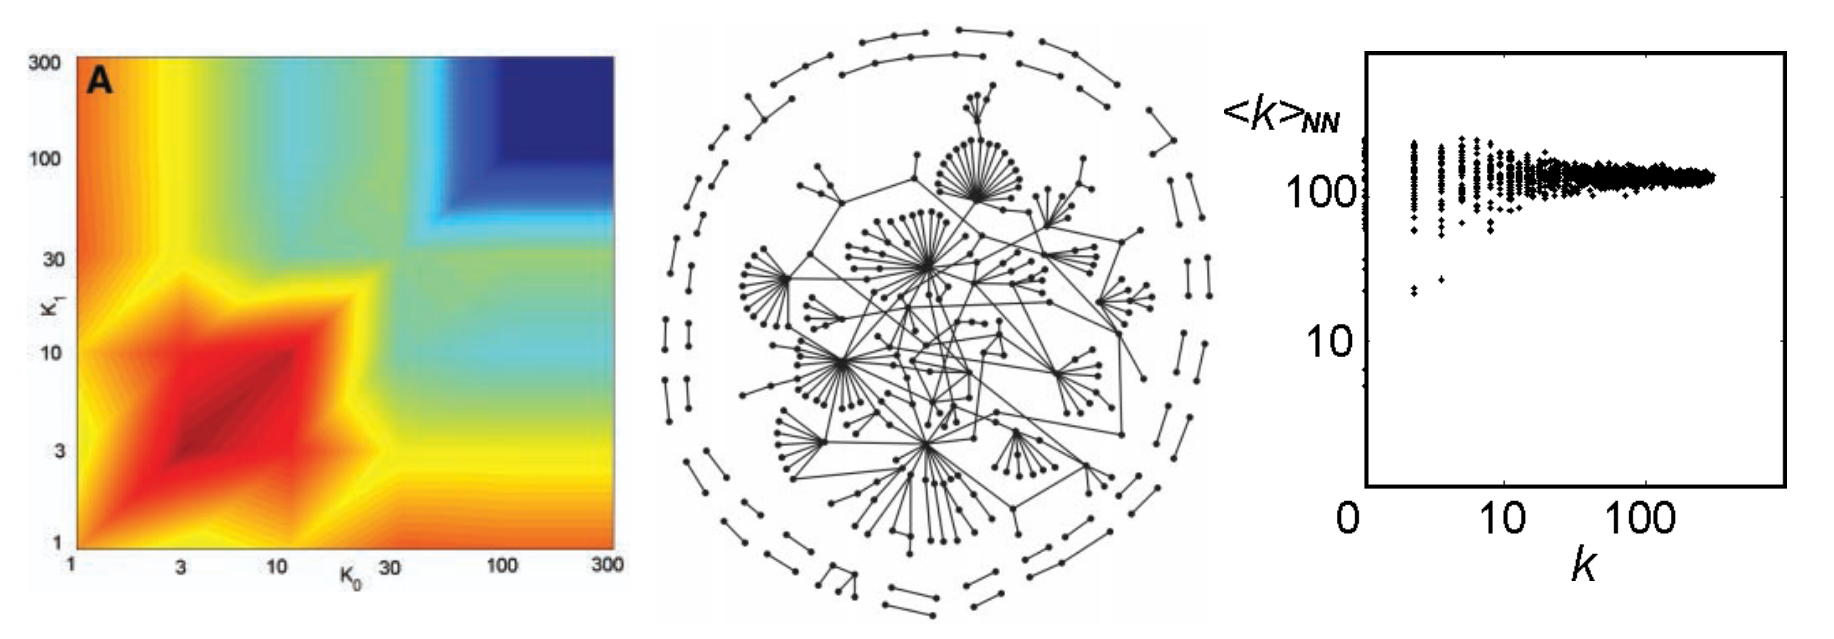
\includegraphics[width=\textwidth]{img/yeast_ppi.png}
        \caption{The Yeast PPI network (Maslov Sneppen Science 2002) shows a non-trivial correlation between \(K_0\) and \(K_1\), as well as for $K$ and $K_{NN}$, which helps identify specialized biological roles. This pattern is destroyed by link reshuffling, indicating it is a product of evolutionary design. In the center we can see a schemaic view of the network, where we can identify "effector" nodes (low degree but high-degree neighbors) and "master" nodes (high degree but low-degree neighbors).}
    \end{figure}
\end{example}

% ==========================================
\subsection{Weighted Networks and Node Strength}
% ==========================================

For weighted networks where links possess a specific \textbf{weight} ($W_{ij} > 0$), the concept of degree is extended to "strength". It should be noted that the degree of a node in a weighted network is still defined as the number of links connected to it, regardless of their weights. However, the strength of a node provides a more nuanced measure of its connectivity by accounting for the weights of the links.

\begin{definition}[Node Strength]
    The strength of a node is defined as the sum of the weights of all links connected to it:
    \[
        S_i = \sum_j W_{ij}.
    \]
\end{definition}

Analyzing the relationship between topological degree ($K$) and strength ($S$) reveals how weights are distributed across the network. Two common patterns are observed:
\begin{itemize}
    \item \textbf{Linear Relationship ($S_i \propto K_i$):} This indicates a random null model where weights are assigned independently of the node's connectivity. In this case, the strength of a node is directly proportional to its degree, suggesting that weights are distributed uniformly across the network.
    \item \textbf{Superlinear Relationship ($S_i \propto K_i^\beta$ with $\beta > 1$):} This indicates a non-random association where highly connected nodes also attract disproportionately heavier weights. A prime example is the US airport weighted network, where weights (traffic) are a function of distances and broader topological metrics.
\end{itemize}

\begin{remark}[Weighted and Topological Networks]
    If we have a weighted network matrix $W$, we can always extract its underlying topological adjacency matrix $A$ by applying an element-wise logical function: $A = W > 0$. Whenever analyzing a weighted network, it is best practice to study the original and the "binarized" (topological) network in parallel to isolate the specific role the weights play: if the weighted and topological analyses yield similar results, then the weights are not adding significant information beyond the topology. Conversely, if the results differ significantly, it indicates that the weights are crucial for understanding the network's structure and function.
\end{remark}

% ==========================================
\subsection{Leafs and Core Networks}
% ==========================================

Nodes with a degree of exactly $K = 1$ are known as pendant nodes, or ``\textit{leafs}''. Conceptually, the number of leafs can be viewed as the network's ``\textit{surface}'', while the total number of nodes represents its ``\textit{volume}''.

We can structurally reduce a network using the \textbf{Pendant Node Removal Algorithm}, which iteratively deletes all nodes with $K=1$. This iterative pruning will result in one of two outcomes:
\begin{enumerate}
    \item \textbf{Nothing remains:} This implies the original network was a pure tree (containing no cycles), where all nodes are leafs except for a few cutpoints. In this case, the network's structure is entirely defined by its degree distribution.
    \item \textbf{A sub-network remains:} We are left with a "core network" without any leafs. In this core, every node has $K \ge 2$, indicating the presence of structural cycles. The properties of this core network are not solely determined by the degree distribution, as the presence of cycles introduces additional structural complexity.
\end{enumerate}

% ==========================================
\section{Closeness Centrality}
% ==========================================

We are going to define the \textbf{closeness centrality} of a node, which is a foundamental measure of the node's importance based on its average distance to all other nodes in the network.

\begin{definition}[Closeness Centrality]
    Closeness is a measure linked to the \textbf{mean shortest path distance} ($P_{ij}$) from one node to all others (\textit{reachability}). The core idea is that a node less distant from all others is more important.
    \[ Cl_i = \frac{N-1}{\sum_{j} P_{ij}} = \frac{1}{\langle P_i \rangle} \]
\end{definition}

Closeness characterizes the \textit{optimal spread capacity of a node} within a few steps—whether it is spreading information, a commodity, or energy. It is a particularly robust measure in systems where there is a probability of \textbf{signal corruption} or information loss at each step along a path. In such cases, the shortest path is not necessarily the most efficient route for spreading, as it may be more susceptible to corruption. Instead, a node with a higher closeness centrality can reach other nodes through multiple paths, increasing the likelihood of successful transmission despite potential losses.

\begin{remark}[Notes on Closeness]
    \begin{itemize}
        \item $Cl_i$ typically exhibits a very small range of values across a network. This is because, in most complex networks, the overall diameter scales logarithmically with the number of nodes, $\log(N)$.
        \item Special care must be taken with disconnected components. If a network is fragmented, the distance to an unreachable node is mathematically infinite, which will break the standard closeness formulation.
        \item Notably, while closeness is calculated for a single local node, its value depends entirely on the global properties of the network.
    \end{itemize}
\end{remark}

\begin{example}[Closeness and Epidemic Spreading]
    Closeness centrality has powerful real-world applications in epidemiology. By combining time series infection data (the onset day of an infection in different regions) with network data representing average human mobility (tracked via mobile phones), researchers can forecast local outbreak timelines. Nodes with higher closeness centrality in the mobility network directly correlate with earlier infection onset days. This relationship is supported by significant Pearson and Spearman correlation values, demonstrating that closeness centrality is a strong predictor of epidemic spread dynamics.

    \begin{figure}[H]
        \begin{minipage}{0.6\textwidth}
            \centering
            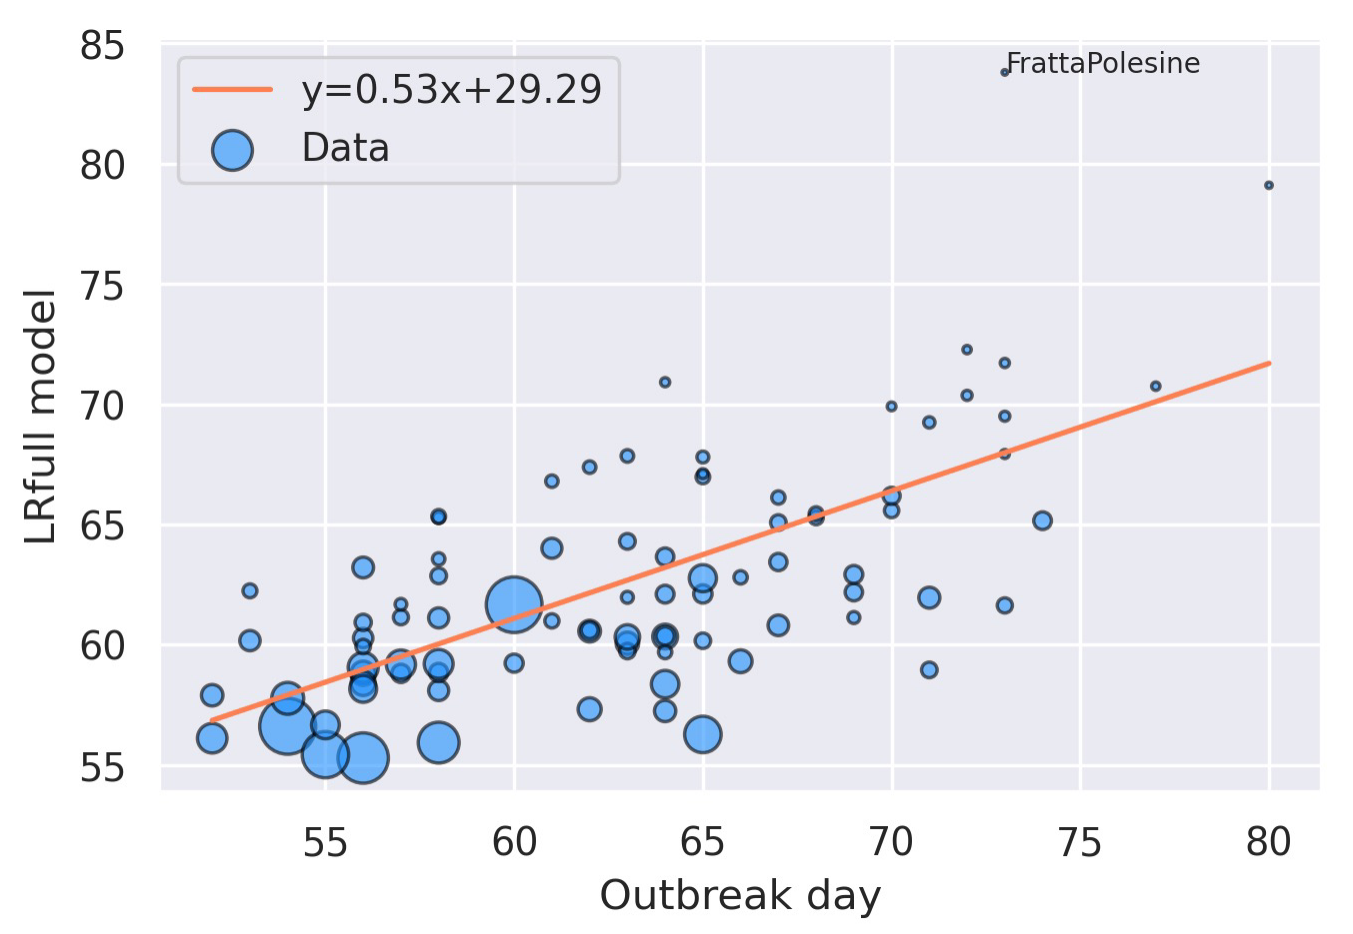
\includegraphics[width=\textwidth]{img/closeness_epidemic-spreading.png}
        \end{minipage}
        \hfill
        \begin{minipage}{0.35\textwidth}
            \caption{Closeness centrality of nodes in a mobility network correlates with the onset day of an epidemic outbreak: nodes with higher closeness centrality experience earlier infection onset, as shown by the significant Pearson and Spearman correlation values.}
        \end{minipage}
    \end{figure}

    \begin{table}[H]
        \centering
        \begin{tabular}{lcccc}
            \toprule
                      & \textbf{Pearson $r$} & \textbf{$r$ p-value} & \textbf{Spearman $\rho$} & \textbf{$\rho$ p-value} \\
            \midrule
            Geo Dist  & $0.276$              & $1 \times 10^{-3}$   & $0.267$                  & $1 \times 10^{-2}$      \\
            Net Dist  & $0.420$              & $5 \times 10^{-5}$   & $0.516$                  & $<1 \times 10^{-6}$     \\
            Closeness & $-0.520$             & $<1 \times 10^{-6}$  & $-0.555$                 & $<1 \times 10^{-6}$     \\
            1/pop     & $0.578$              & $<1 \times 10^{-6}$  & $0.548$                  & $<1 \times 10^{-6}$     \\
            \bottomrule
        \end{tabular}
        \caption{Correlation between infection outbreak day and different distance/centrality metrics.}
        \label{tab:closeness_epidemic}
    \end{table}
\end{example}




% ==========================================
\section{Betweenness Centrality}
% ==========================================

\begin{definition}[Betweenness Centrality]
    % Define for nodes and edges (intermediation/traffic).
    \[ BC_i = \frac{\#P_{mn}(i)}{\#P_{mn}} \]
\end{definition}

\subsection{Normalized Betweenness}
% Explain scaling with respect to the maximum BC value (star network).
\[ BC_{MAX} = \frac{(N-1)(N-2)}{2} \]
\[ BC_{ABS} = \frac{BC}{BC_{MAX}} \]

\subsection{Betweenness and Global Efficiency}
% Define Global Efficiency (harmonic composition) and its relation to BC.

\begin{example}[Immune System Network Analysis]
    % Discuss the bipartite directed graph of cells and mediators.
    % Explain the perturbative effect of mediator removal on Global Efficiency.
    \TODO{Add image of Immune System bipartite network and mediator ranking plot}
\end{example}

% ==========================================
\section{Eigenvector Centrality}
% ==========================================

\begin{definition}[Eigenvector Centrality]
    % Relate to being connected to other "important" nodes.
    \[ EC_i \propto \sum_{j \sim i} EC_j \implies A \vec{x} = \lambda \vec{x} \]
\end{definition}

\subsection{Directed Networks: Hubs and Authorities}
% Explain right eigenvector (pointed by others) vs left eigenvector (pointing to others).

\begin{definition}[Hubs and Authorities (HITS)]
    % Define Authorities (x) and Hubs (y).
    \[ \vec{x} = \alpha A \vec{y}, \quad \vec{y} = \beta A^T \vec{x} \]
    \[ AA^T \vec{x} = \lambda \vec{x}, \quad A^T A \vec{y} = \lambda \vec{y} \]
\end{definition}

% ==========================================
\section{Network Backbone and Salient Links}
% ==========================================

\begin{definition}[Salient Links]
    % Define via spanning trees of shortest paths.
    \[ S = \langle T \rangle = \frac{1}{N} \sum_k T_k \]
\end{definition}

\subsection{Difference Between Salience and Betweenness}
% Explain spontaneous stratification and the bimodal distribution of salient links in weighted graphs.
\TODO{Add images comparing Link Weight, Link Betweenness, and Salience distributions (Air traffic, Food web, etc.)}
\TODO{Add image showing BC vs Salience in a planar graph}

% ==========================================
\section{Clustering Coefficient}
% ==========================================

\begin{definition}[Clustering Coefficient]
    % Define transitivity / 3-cycles.
    \[ C_i = \frac{2e_i}{k_i(k_i - 1)} = \frac{\#C_3}{\#C_2} \]
\end{definition}

\subsection{Clustering Coefficient in Erdős-Rényi Networks}
% Explain the E-R null model limit.
\[ \lim_{N \to \infty} C_G = 0 \quad (\text{for constant } \lambda) \]

\begin{example}[Clustering in Brain Networks]
    % Discuss functional NMR, correlation matrices, and thresholds leading to high transitivity.
\end{example}

% ==========================================
\section{Statistical Properties in Null Models}
% ==========================================

\subsection{Types of Null Models}
% Briefly define Global, Local, and Meso-scale null models.

\subsection{Gaussianity of Centrality Measures in E-R}
% Discuss how centrality measures distribute in large random graphs.
\TODO{Add quantile plots showing Gaussianity of Closeness, Eigenvector, and Betweenness centralities}

\subsection{Scaling Relations: Degree vs. Betweenness}
% Explain the exact limit for a tree vs generic networks.
\[ BC \le K^2 \]
\TODO{Add scatterplots of Closeness vs K, BC vs K, and EC vs K for E-R graphs}
\TODO{Add diagram of tree-structure regions explaining the $BC \propto K^2$ limit}

% ==========================================
\section{Comparative Examples in Basic Topologies}
% ==========================================
% Section to visualize how K, BC, CL, and EC behave in simple, deterministic graphs.

\begin{example}[Complete Graph]
    \TODO{Add graph drawing and centrality values table/plot for a complete graph}
\end{example}

\begin{example}[Path Graph]
    \TODO{Add graph drawing and centrality values table/plot for a path graph}
\end{example}

\begin{example}[Cycle Graph]
    \TODO{Add graph drawing and centrality values table for a cycle graph}
\end{example}

\begin{example}[Dumbbell and Block Networks]
    % Compare structural holes, cutpoints, and redundant cutpoints.
    \TODO{Add graph drawings and centrality values tables/plots for block networks and generic trees}
\end{example}